\section{Background: RP}
\label{background}
\label{nutshell}

Reactive Programming (RP) is a declarative programming paradigm for working with streams of input data. 
According to the first definition\footnote{
``Reactive programs [..] maintain a continuous interaction with their environment, at a speed which is determined by the environment, not the program itself.''~\cite{berry1989real}
} a reactive program must interact with the environment `at a speed which is determined by the environment'.
Conceptually, when a reactive program is run, it sets up a data pipeline and waits until input arrives when the environment changes.
Reactive Programming languages and libraries provide developers with a set of abstractions and methods to create such programs.

The programming paradigm of Reactive Programming is implemented by multiple languages and libraries. 
Many RP implementations share a notion of a collection that abstracts over \emph{time}, in contrast to \emph{space} like standard collections.
This collection comes in different flavors, 
such as Observable (Rx~\cite{meijer2010subject}), 
Signal (Elm~\cite{czaplicki2012elm}), 
Signal/Event (REScala~\cite{salvaneschi2014rescala}) or 
Behavior/Event (FRP~\cite{elliott1997functional}).
The implementations differ in the precise semantics of their collections, their execution model (push/pull), and the set of available operators.  
In this paper, we focus on the Rx formulation, but our work is applicable to other RP implementations to some extend. 

Understanding how we arrive at our visualization requires a minimal understanding of Rx.
Rx introduces two basic types \emph{Observable} and \emph{Observer}. Observables define the data flow and produce the data while Observers receive the data, possibly moving the data further down the stream. Figure \ref{sample1} shows a very basic example of an ``in situ'' data flow in Rx. Initially, an Observable is created, here using the static \code{of} method, then dependent Observables are created using the \code{map} and \code{filter} methods on the Observable instance. Finally we \code{subscribe} to start the data flow and send the data in the flow to the console.

\begin{figure*}[h!]
\centering

\begin{subfigure}[t]{\columnwidth}
	\inputminted[tabsize=2]{javascript}{listings/sample1.js}	
	\par\bigskip
	\caption{Rx code example}
	\label{sample1}
	\par\medskip
	\begin{tikzpicture}[->,>=stealth',shorten >=1pt,auto,node distance=2.8cm,
                    semithick,scale=0.8, every node/.style={scale=0.8}]
  \tikzstyle{every state}=[]

  \node[state] (A)                    {$o_1$};
  \node[state] (B) [right of=A]       {$o_2$};
  \node[state] (C) [right of=B]       {$o_3$};

  \node[state] (X) [below right =1cm of A] {$s_3$};
  \node[state] (Y) [right of=X]            {$s_2$};
  \node[state] (Z) [right of=Y]            {$s_1$};

  \path (B) edge   node {source}                   (A)
        (C) edge   node {source}                   (B)
        (A) edge [bend left] node {map(\_ * 2)}    (B)
        (B) edge [bend left] node {filter(\_ < 3)} (C)
        (X) edge   node[below] {destination}       (Y)
        (Y) edge   node[below] {destination}       (Z)
        (Z) edge   node {subscribe}                (C)
        (Y) edge   node {subscribe}                (B)
        (X) edge   node {subscribe}                (A);

  \draw[<-] (A) -- node[above] {of(1,2,3)} ++(-2cm,0);
  %\draw[<-] (Z) -- node[below] {subscribe} ++(2cm,0);

\end{tikzpicture}

	\caption{Rx graph example}
	\label{chaincreate}
\end{subfigure}
\begin{subfigure}[t]{\columnwidth}
	\inputminted[tabsize=2]{javascript}{listings/sample3.js}	
	\caption{Higher order flatMap operation}
	\label{sample3}
	\par\medskip
	\begin{tikzpicture}[->,>=stealth',shorten >=1pt,auto,node distance=2.8cm,
                    semithick,scale=0.8, every node/.style={scale=0.8}]
  \tikzstyle{every state}=[]

  \node[state] (A)                    {$o_2$};
  \node[state] (B) [right of=A]       {$o_3$};
  \node[state] (C) [right of=B]       {$o_4$};

  \node[state] (X) [below right =1cm of A] {$s_3$};
  \node[state] (Y) [right of=X]            {$s_2$};
  \node[state] (Z) [right of=Y]            {$s_1$};
  
  \node[state] (F) [below =2cm of B]              {$o_1$};
  \node[state] (P) [below =1.8cm of Y] {$s_{4,n}$};
  \node[state] (Q) [below =0.3cm of P]       {$s_{4,m}$};

  \path (B) edge   node {source}                   (A)
        (C) edge   node {source}                   (B)
        (A) edge [bend left] node {skip(1)}    (B)
        (B) edge [bend left] node {flatMap(() => inner)} (C)
        (X) edge   node[below] {destination}       (Y)
        (Y) edge   node[below] {destination}       (Z)
        (Z) edge   node {subscribe}                (C)
        (Y) edge   node {subscribe}                (B)
        (X) edge   node {subscribe}                (A)
        
        (P) edge [bend right]  node[sloped,above] {subscribe}   (F)
        (P) edge   node[sloped,below] {destination} (Z)
        (Q) edge [bend left]  node[sloped,above] {subscribe}   (F)
        (Q) edge   node[sloped,below] {destination} (Z);
  
%  \node[draw=none] (K) at ($ (P) + (-4:-3) $){$\cdots$};
%  \node[draw=none] (M) at ($ (Q) + (-4:-3) $){$\cdots$};  
        
  % https://tex.stackexchange.com/questions/75497/automata-container-box
  \node [draw=red, label={\color{red}inner}, fit=(F) (P) (Q), inner sep=0.5cm,dashed, ultra thick, fill=red!10, fill opacity=0.2] {};
  %\node [draw=blue, fit= (G) (Q) (M), inner sep=0.5cm,dashed, ultra thick, fill=blue!10, fill opacity=0.2] {};

  % https://tex.stackexchange.com/questions/160643/ellipsis
  \draw[<-] (A) -- node[above] {of(1,2,3)} ++(-2cm,0);
  \draw[->] (F) -- node[above] {$\cdots$} ++(-2cm,0);
  \draw[<-] (P) -- node[above] {$\cdots$} ++(-3cm,0);
  \draw[<-] (Q) -- node[above] {$\cdots$} ++(-3cm,0);

\end{tikzpicture}

	\caption{Higher order Rx graph example}
	\label{chainhigher}
\end{subfigure}

\caption{Samples of Rx Observables}

\end{figure*}

\paragraph{Assembly} It is important to note that Observables are lazy; initially they only specify the blueprint of a data flow. 
Creating this specification is called the \emph{assembly} phase. In the code sample of Figure \ref{sample1} the assembly phase consists of the calls to \code{of}, \code{map} and \code{filter}, creating respectively Observables $o_1$, $o_2$ and $o_3$ from Figure \ref{chaincreate}.

\paragraph{Subscription} When the \code{subscribe} method of an Observable is called, the data flow is prepared by recursively subscribing up the stream: every subscribe call creates an \emph{Observer}, that is passed to the input Observable, which again subscribes an Observer to its input Observable, until finally the root Observables are subscribed to. We call this the \emph{subscription} phase. In Figure \ref{sample1} inside the single \code{subscribe} call Observer $s_1$ from Figure \ref{chaincreate} is created and passed to $o_3$, which in turn will recursively subscribe to $o_2$ with a new Observer $s_2$ with destination $s_1$, until the full chain is subscribed.

\paragraph{Runtime} After the root Observables are subscribed to, they can start emitting data. This is the \emph{runtime} phase. Depending on the nature of the Observable this might attach event listeners to UI elements, open network connections or start iterating over a list of elements. Events are pushed to $s_3$, to $s_2$ and finally to $s_1$ which calls \code{console.log} in Figure \ref{sample1}. 

Rx identifies three types of events that can occur during the runtime phase: `next', `error' and `complete'-events. Next-events contain the next value in the flow, an error-event encapsulates an error and is a unsuccessful termination to a stream, while a complete-event denotes the successful termination of the stream. There are restrictions on their order: a Observable may first emit an unlimited amount of next-events, and then either an error or a complete event. Observables do not need to emit any next-events, and do not need to terminate.

More complex programs feature operators that merge Observables\footnote{
	\code{concat}, \code{merge}, \code{combineLatest}, \code{zip}
}, split Observables\footnote{
	\code{partition}, or through sharing with \code{share} or \code{publish}
} or handle higher order Observables\footnote{
	\code{flatMap}, \code{mergeMap}, \code{concatMap}
}, resulting in more complex graphs. While merging and splitting happens on an Observable level (the \code{source} property still points to the one or more dependencies) higher order Observable flattening manifests only in Observer structure (there is no reference between the Observables). Figure \ref{chainhigher} shows this with an (abbreviated) \code{inner} Observable that is subscribed twice (for both values $2$ and $3$, value 1 is skipped), resulting in two identical data flows over $o_1$. The data flow through $s_{4,n}$ and $s_{4_m}$ is pushed into $s_1$, flattening the data flow. 

\begin{figure}[t]
\centering
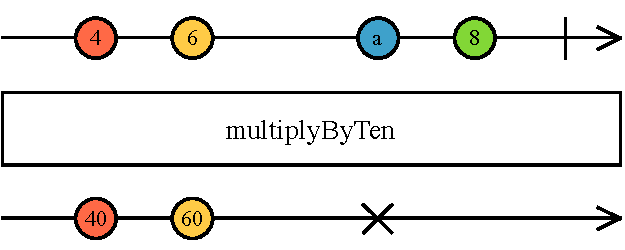
\includegraphics[width=\columnwidth]{images/marble-diagram.pdf}
\caption{Marble Diagram}
\label{marblediagram-image}
\end{figure}

\paragraph{Marble Diagram}
\label{marblediagram}
The term \textit{Marble Diagram} comes from the shape of the glyps in the images used to explain Rx in the official documentation. An example is shown in Figure~\ref{marblediagram-image}.
The diagrams contain one or more timelines containing the events that enter and leave Observables. 
Next-events are typically represented with a circle, an error-event with a cross and a complete-event with a vertical line.
Developers can see from the diagram how operators work by inspecting the difference between the timelines, 
where events might be skipped, added, transformed or delayed. 
Mapping time on the x-axis provides insight that is missing when inspecting only a single time slice. 